\documentclass[10pt,twocolumn]{article}
\usepackage[letterpaper,top=0.70in,bottom=0.72in,left=0.68in,right=0.68in,columnsep=0.24in]{geometry}
\usepackage{newtxtext,newtxmath}
\usepackage{graphicx}
\usepackage{booktabs}
\usepackage{tabularx}
\usepackage{array}
\usepackage{enumitem}
\usepackage{microtype}
\usepackage{fancyhdr}
\usepackage{titlesec}
\usepackage{xcolor}
\usepackage{url}
\usepackage{caption}
\setlength{\parindent}{1em}
\setlength{\parskip}{0pt}
\setlist{nosep,leftmargin=*}
\pagestyle{fancy}
\fancyhf{}
\fancyhead[L]{\small The Equal SQLs, CSC312 2026}
\fancyhead[R]{\small AgriCare: Prototype Development}
\fancyfoot[C]{\small \thepage}
\renewcommand{\headrulewidth}{0pt}
\titleformat{\section}{\large\bfseries}{\thesection}{0.5em}{}
\titleformat{\subsection}{\normalsize\bfseries}{\thesubsection}{0.45em}{}
\captionsetup{font=small,labelfont=bf}
\setcounter{page}{9}
\setcounter{section}{6}
\begin{document}

\section{PROTOTYPE DEVELOPMENT}
\subsection{Purpose and Scope}
Step 5 converts the analysis models from the previous deliverable into executable program code. The prototype is intentionally a \emph{vertical slice}: instead of attempting every requirement at once, it implements a small set of high-value workflows end-to-end so that the code can be extended into the completed AgriCare application. The implemented slice is traced directly to the Step 4 use cases and functional requirements: animal profiles (UC01), vaccinations and booster due dates (UC02), illness reporting and severity classification (UC03), quarantine transitions (UC04), a role-specific dashboard (UC08), outbreak flagging as an early version of UC06, and audit logging (UC10).

The prototype keeps the domain rules established during requirements analysis. For example, a red-flag symptom is classified as Urgent, Moderate or Urgent reports can place a healthy animal into Suspect status, quarantine transitions are constrained by the state model, and only the Veterinarian demo role can record vaccinations or change quarantine state. These rules are implemented on the server rather than only in the interface, so changing the user interface later does not remove the validation.

\subsection{Prototype Architecture}
Figure~\ref{fig:architecture} shows the current structure. The browser interface communicates with a FastAPI REST layer using JSON. The API validates input and role permissions before calling domain rules. SQLAlchemy isolates persistence from the API. For demonstration the default database is SQLite because it can run on any group member's laptop without database-server configuration; the same code can target MySQL by setting the \texttt{DATABASE\_URL}. MySQL remains the database selected for the completed system.

\begin{figure}[ht]
\centering
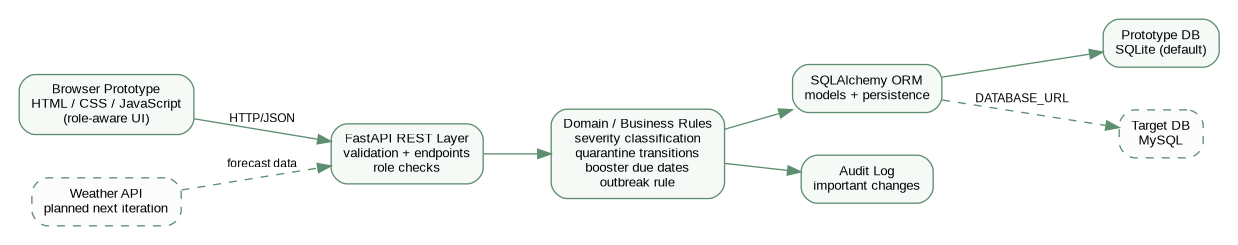
\includegraphics[width=\columnwidth]{architecture.png}
\caption{Step 5 program-code prototype architecture. Dashed components indicate the target MySQL database and planned weather-service integration.}
\label{fig:architecture}
\end{figure}

\subsection{Hardware and Software Environment}
No specialist hardware is required for the current prototype. A normal student or laboratory computer with an x64 processor, at least 4~GB RAM, approximately 500~MB free storage, and a modern browser is sufficient. Internet access is not required for the core local demo; it will become necessary when the weather API and hosted deployment are added. The interface is responsive so that the same prototype can be demonstrated on a laptop and tested at mobile widths.

\begin{table}[ht]
\caption{Step 5 development environment and toolchain.}
\label{tab:stack}
\small
\begin{tabularx}{\columnwidth}{>{\bfseries}p{0.27\columnwidth}X}
\toprule
Area & Prototype choice and purpose \\
\midrule
Backend & Python with FastAPI for REST endpoints, validation and business rules. \\
Persistence & SQLAlchemy ORM; SQLite for the portable prototype and MySQL as the target database. \\
Frontend & HTML, CSS and JavaScript browser prototype, separated from the API so it can be replaced by the planned React interface without changing backend contracts. \\
Testing & \texttt{pytest} for automated rule tests; Postman or command-line HTTP requests for endpoint checks. \\
Database tools & MySQL Workbench when the MySQL configuration is enabled. \\
Version control & Git/GitHub for source control, review and change history. \\
Design/docs & Existing UML models, Figma/Draw.io artefacts and the ACM-format report continue to guide implementation. \\
\bottomrule
\end{tabularx}
\end{table}

\subsection{Implemented Key Functionality}
Table~\ref{tab:trace} records what has moved from requirement to executable code. The purpose is not to claim that Step 5 is the completed product; it establishes a working base around which later sprints can add treatment records, weather integration, notifications, complete authentication, security incidents and the remaining nice-to-have requirements.

\begin{table*}[t]
\caption{Traceability from Step 4 requirements to Step 5 prototype evidence.}
\label{tab:trace}
\small
\begin{tabularx}{\textwidth}{p{0.13\textwidth}p{0.21\textwidth}X p{0.20\textwidth}}
\toprule
Requirement & Prototype function & Executable behaviour & Evidence in code/UI \\
\midrule
UC01; FR-02--04 & Animal profiles & Create, list and open active animal files identified by unique tag ID; duplicate tag IDs are rejected. & \texttt{/api/animals}; Animals screen \\
UC02; FR-05--06 & Vaccination & Veterinarian records vaccine data; next booster due date is calculated from administration date plus interval. & \texttt{/vaccinations}; Clinical Actions screen \\
UC03; FR-07 & Illness report & Symptoms are saved and classified Low, Moderate or Urgent. Red-flag symptoms become Urgent. & \texttt{/illness}; automated rule tests \\
UC04; FR-08 & Quarantine & Veterinarian-only transitions are checked against Healthy $\rightarrow$ Suspect $\rightarrow$ Isolated $\rightarrow$ Monitored $\rightarrow$ Cleared, with permitted backward transitions only. & \texttt{/quarantine}; transition table in code \\
UC06; FR-10 & Outbreak flag & Early rule counts distinct animals with reports in the same enclosure/body system during a 72-hour window; three or more creates an alert. & \texttt{OutbreakAlert}; dashboard count \\
UC08; FR-12 & Dashboard & Shows total animals, animals in quarantine, urgent reports, overdue vaccination records and open outbreak flags. & Dashboard page and \texttt{/api/dashboard} \\
UC10; FR-14 & Audit trail & Important create/report/vaccination/quarantine actions write an audit record; access to the log is role-limited. & \texttt{AuditLog}; Audit Trail screen \\
NFR-02/04/09 & Security, integrity, maintainability & Server-side role checks, duplicate/transition validation and separated database/model/schema/API modules. & Backend modules and 403/400 responses \\
\bottomrule
\end{tabularx}
\end{table*}

\begin{figure*}[t]
\centering
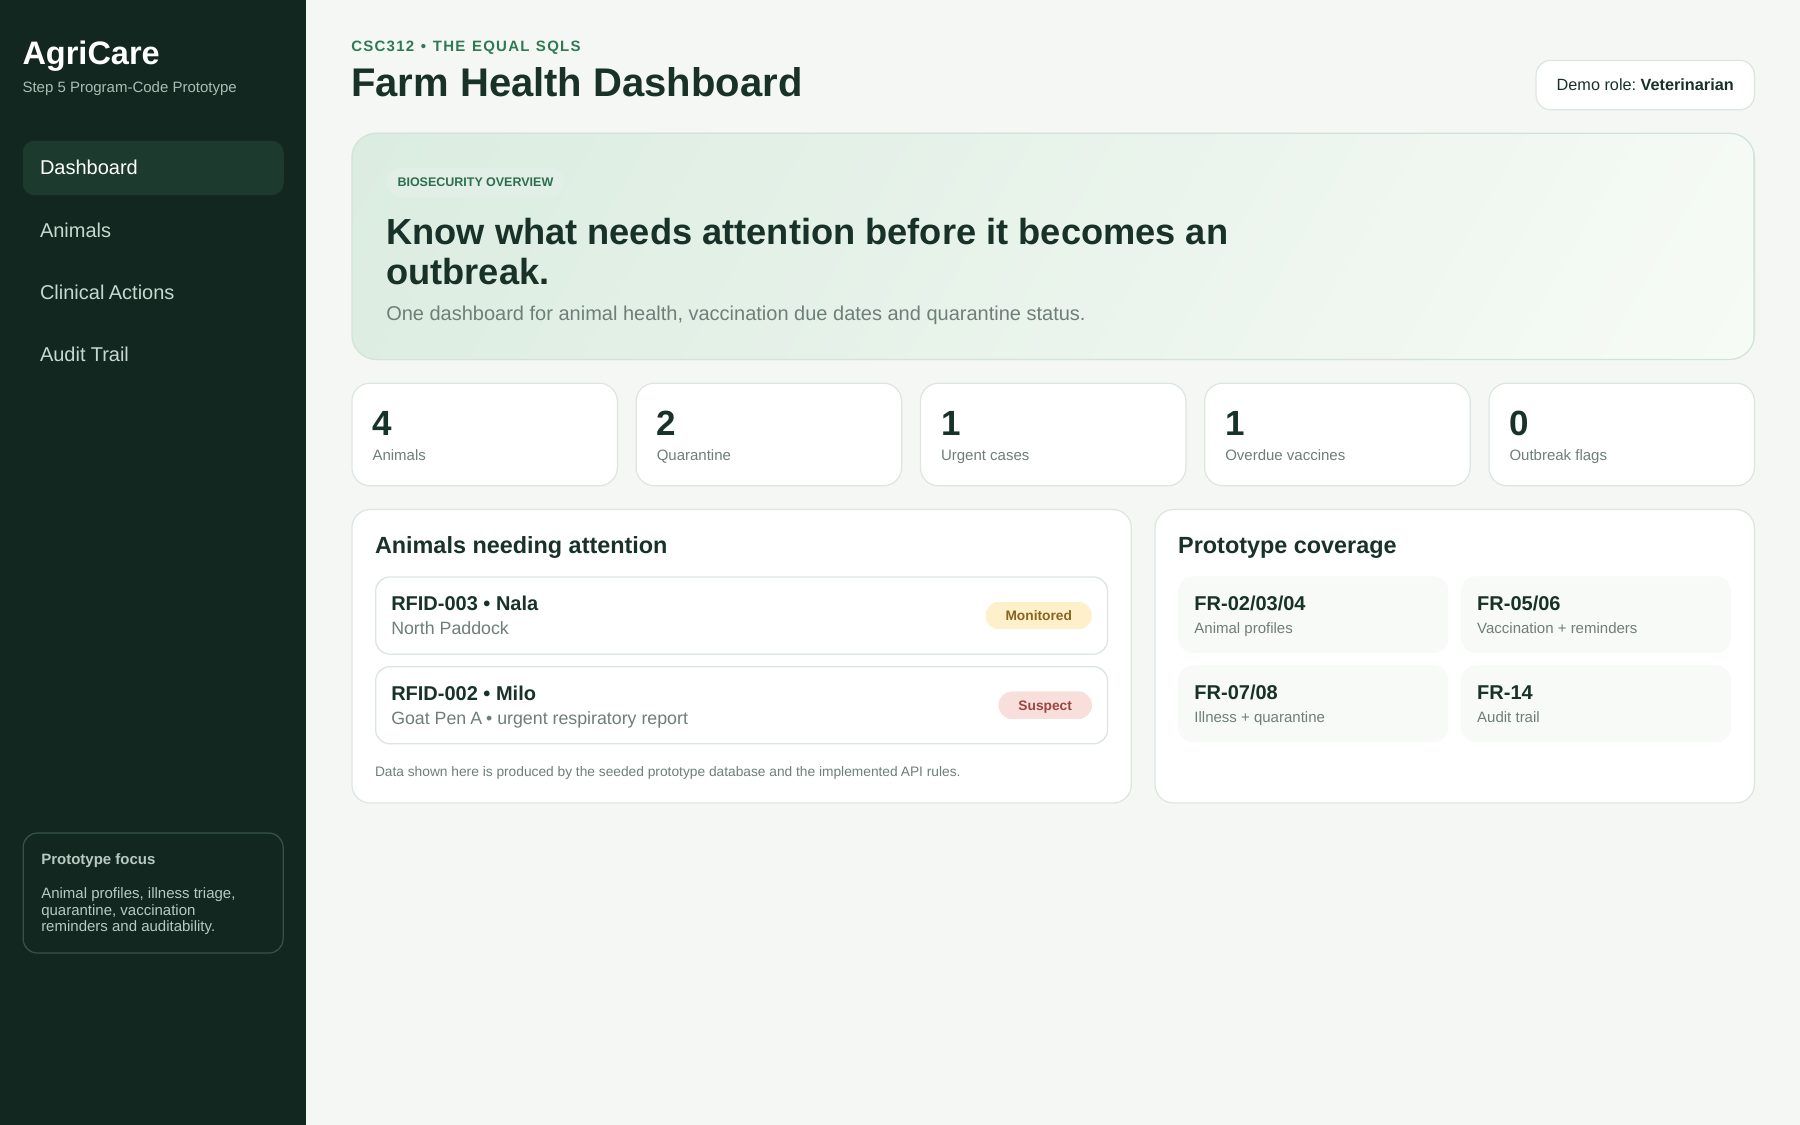
\includegraphics[width=0.93\textwidth]{screenshots/prototype_dashboard.png}
\caption{Dashboard view of the runnable Step 5 prototype. The interface follows the Step 4 ``notice board'' mental model and exposes the implemented vertical slice.}
\label{fig:prototype}
\end{figure*}

\subsection{Prototype Data and Behaviour}
The data model used in code is a deliberately smaller implementation of the high-level Step 4 class diagram. The prototype persists \texttt{Animal}, \texttt{IllnessReport}, \texttt{VaccinationRecord}, \texttt{QuarantineEvent}, \texttt{OutbreakAlert} and \texttt{AuditLog}. Foreign-key relationships link clinical events to the animal file. This allows the application to show one animal's history while keeping event records independently auditable.

Several behavioural rules from Step 4 are now executable. The severity function treats breathing difficulty, collapse, mouth lesions, hoof lesions or sudden death as red flags. Fever or two or more non-red-flag symptoms produces Moderate severity, otherwise the result is Low. A Moderate or Urgent report on a Healthy animal creates a Suspect transition. Vaccination due dates are calculated rather than manually typed. The quarantine API checks each requested state change against the permitted transition set and rejects an invalid jump such as Healthy directly to Cleared.

\subsection{Verification of the Prototype}
Testing is part of the prototype rather than an activity postponed until the final product. Five automated unit tests currently exercise severity classification, quarantine transition rules and booster-date calculation. All five pass in the supplied code. Manual API checks were also performed for the main access-control path: a Care Staff request to record a vaccination receives HTTP 403, while the same valid request under the Veterinarian role is accepted and the next due date is calculated. An Urgent illness report was also verified to return Urgent severity and place the animal into Suspect status.

\begin{table}[ht]
\caption{Current Step 5 verification evidence.}
\small
\begin{tabularx}{\columnwidth}{p{0.23\columnwidth}X p{0.16\columnwidth}}
\toprule
Check & Expected result & Result \\
\midrule
Rule tests & 5 tests pass & Pass \\
Red flag & ``breathing difficulty'' $\rightarrow$ Urgent & Pass \\
Access control & Care Staff vaccination request rejected & 403 \\
Vaccination & 365-day interval computes next due date & Pass \\
Transition & Healthy $\rightarrow$ Cleared rejected & Pass \\
\bottomrule
\end{tabularx}
\end{table}

Performance targets such as the 300~ms requirement have not yet been formally load-tested, so Step 5 does not claim compliance with those targets. They remain acceptance criteria for a later sprint when the MySQL and deployment environments are stable.

\section{CONTINUED APPLICATION OF SOFTWARE ENGINEERING ASPECTS}
\subsection{Process}
The group continues to use Agile/Scrum. Step 4 use cases and requirements act as the product backlog; Step 5 selects a small vertical slice of the must-have backlog for implementation. The practical sprint cycle is: select backlog items, refine acceptance criteria, implement the smallest working path, test it, review the result against the requirement, and return incomplete or newly discovered work to the backlog. The prototype therefore becomes an evolutionary base rather than disposable code.

\subsection{Principles}
\textbf{Separation of concerns} is visible in the code structure: database setup, ORM models, validation schemas, domain rules, HTTP endpoints and browser assets are separated. This reduces coupling and makes the planned React migration possible without rewriting domain rules. \textbf{Least privilege} is applied by checking the role at server endpoints; for example only the Veterinarian demo role may record vaccinations or change quarantine state, while audit viewing is limited to audit-relevant roles. \textbf{Defence in depth} is only partially implemented at prototype level: server-side checks exist even if an interface control is hidden, but production authentication, HTTPS, secure credential storage and full authorisation remain future work. \textbf{Data integrity} is supported through required fields, unique animal tags, foreign keys and rejected invalid state transitions.

\subsection{Methods and Techniques}
The prototype continues the selected methods of UML-guided development and Test-Driven Development. The use-case and state models are translated into endpoints and executable transition rules, preserving traceability from analysis to code. Rule tests are written around behaviours that are easy to break, such as severity and quarantine progression. API-based prototyping also gives the group a stable interface contract: the browser client can later be replaced with React while calling the same endpoints.

\subsection{Software Quality Goals}
The ISO/IEC 25010-oriented goals from the previous report continue to guide implementation. \textbf{Functional suitability} is addressed by tracing each implemented function to a requirement. \textbf{Usability} is addressed through short forms, a role selector for demonstration, a dashboard-first layout and plain-language status labels. \textbf{Accessibility} is supported by pairing words with status colour and using responsive controls. \textbf{Security} is represented by server-side role checks, while the current header-based role simulation is explicitly not treated as production authentication. \textbf{Reliability/integrity} is supported by input validation and fail-fast error responses. \textbf{Maintainability} is supported by modular source files and automated tests. \textbf{Compatibility} is supported through a browser-based interface and JSON API, with MySQL configuration kept outside code through an environment variable.

\subsection{Umbrella Activities}
Configuration management continues through version control and a source tree that can be reviewed by all group members. Technical reviews compare each implementation with its originating requirement and use-case flow. Risk management is updated as implementation reveals new risks: the most important current risks are prototype authentication being mistaken for final security, database migration differences between SQLite and MySQL, false positives from the simple outbreak rule, and schedule pressure from unimplemented weather/treatment functionality. Documentation is kept with the code in a README and requirement-traceability file. Measurement currently includes test pass/fail results and implemented-requirement coverage; later sprints will add performance measurements and defect counts.

\subsection{Tools in the Step 5 Workflow}
FastAPI and Python implement the service layer; SQLAlchemy provides database independence; SQLite provides a zero-configuration demonstration database while MySQL remains the final target. HTML/CSS/JavaScript implements the current program-code interface, with React planned as the evolved front end. \texttt{pytest} supports automated tests, Postman or command-line requests support API verification, MySQL Workbench supports the final database, Git/GitHub supports source control and collaboration, Figma supports interface refinement, Draw.io supports UML and architecture updates, and Word/LaTeX/PDF tooling supports the ACM-format documentation.

\section{PROTOTYPE LIMITATIONS AND EVOLUTION PLAN}
The current prototype deliberately does not represent the completed AgriCare system. The role selector sends a demonstration role header instead of performing secure authentication; this must be replaced with registered users, password hashing and server-managed identity. Weather integration, treatment records, security-incident workflows, notification delivery, full archive/update operations, richer outbreak confirmation and the remaining nice-to-have requirements are not yet complete. The final database should be exercised with MySQL, and the user interface should be migrated to React as planned in the proposal.

The next sprint should therefore (1) implement secure login and user/role persistence, (2) migrate and test the schema on MySQL, (3) add treatment history and complete animal editing/archive operations, (4) integrate a weather provider behind a service interface with cached fallback data, (5) convert the current browser views into React components, and (6) run usability, accessibility and performance tests against the measurable NFR targets. This keeps Step 5 code as the foundation of the completed application rather than replacing it with a new implementation.

\end{document}
